
\section{Introduction}

Online fashion market has been growing rapidly every year. Clothing purchasing decisions are very difficult without personal try-on experience. The current non-customized information, like the cloth and models' try fit images are not enough to know how well the cloth matches with her or him.   
%Unlike other products, such as electronic devices, whose function, performance, and styles can be expected through few images and specification tables. Fashion apparels have infinite variations in style, forms, colors, texture, and materials.  Also the difference between personal preferences is huge. 
Therefore, virtual try-on (VTON) is a highly demanding technology for the on-line shopping\cite{zhang2019role}. 

The early VTON technologies were based on 3D computer graphics technology that uses 3D models of target humans and clothing. However, the 3D models are usually  difficult or expensive to obtain. Therefore, recently 2D image-based VTON technologies are being studied in academia and industry, powered by the recent advances in computer vision technologies based on deep learning. 

There have been many related studies to image-based VTON. They assumes diverse input condition and problem settings, from clothed human pose transferring using conditional GAN \cite{ma2017pose}, swapping two humans clothes \cite{jetchev2017conditional}, to VTONs with a try-on cloth and a target human image \cite{Han2017VITONAI}. The last problem settings with a try-on cloth and a target human image has been considered practical in many papers, \cite{Han2017VITONAI,Wang2018TowardCI}, and more recently \cite{Sun2019ImageBasedVT,Yu_2019_ICCV,jae2019viton}. I this paper, we also consider this setting. The commonly-used processing pipeline for this setting divides the problems into to stages: First, it warps the try-on cloth to align it with the target human, and then blends the warped cloth with the
target human image. In some papers, the warping and blending stages are called Geometric Matching Module (GMM) and Try-On Module (TOM), respectively. In this work, we will use the two expressions interchangeably.


%In this paper, we also consider the VTON problem that use the try-on cloth and human images and generated a new virtual image that the target human replaced the current top or bottom cloth with the try-on cloth. Our implementation is also limited to top clothes due to the restricted dataset but the bottom clothes, e.g. pants or skirts would be easier than top cloth cases because they are simpler than upper clothes in style and shapes.

Although the previous studies demonstrate the feasibility of image-based VTON technology, our experiment with classified inputs on the cloth styles and human posture in the Section \ref{section_comparsion} reveals serious problems and challenges in the image-based approach. 
Even though the neural network systems are criticized for its black-box system properties, 
%at least the real design of network structure, input data, and training mechanism are based upon the understanding on the cause-and-result relations. 
we demonstrates the examination of results based on the classified inputs and  cause-and-result reasoning can still help understand and improve the network and methods and systems. The experimental results show that the state-of-the-art methods work fairly well for the cases of  mono-colored short-sleeved clothes and an up-front posed human, but not for the cases with a rich-textured and long-sleeved cloth or a diverse posed human.    
Also, we demonstrate the examination at intermediate results in the multi-stage pipeline system is an effective tool for understanding the limitations and the operating ranges of the algorithms. 

This classified examination and observation helps us to design a modification of warping network, a better input processing, and new training methods. First we find and correct the erroneous cloth-agnostic human representation: the wrong labeling of the chest area and missing parts not to replace in VTON process. Second, we observed the problem in cloth warping networks: the unbalanced geometric matching inputs and training loss function. Finally, we improve the composition mask using input cloth mask and concrete loss function.   The proposed system, name CP-VTON+ after its base CP-VTON outperforms its base algorithm quantitatively and qualitatively: in Intersection-Over-Union (over 10 percent) and Structural Similarity Index (over 7 percent) for the same cloth re-try-on, and Inception Score and visual observation (over 4 percent) for new cloth try-on test. 

The contributions of this work are three-fold. First, we provide the detailed performance evaluations of the existing Image-based algorithms with classified input conditions. Second, the limitation and operating range of the previous algorithm and more generally 2D image based VTON approaches are clearly identified and the origin of limitations are explained together with  the reason why the previous works seemingly work well with the used dataset. Finally, a new pipeline is proposed to tackles the identified problems. Experiments show the proposed pipeline can solve the problems and how much the problem affects the performance. 

   
% We would emphasize here that one reason of the seemingly high quality in the existing algorithms are mainly due to the dataset with low-complexity bias, i.e., most clothes are short-sleeved  and monochromatic, and the poses of humans are mostly in an up-right position. Specifically, as it will be shown in the following section, the results with the long-sleeved cloth arm and body posed shows very low quality. In Section 3, we point out serious problems in previous methods.


%\begin{figure}
%\centering
%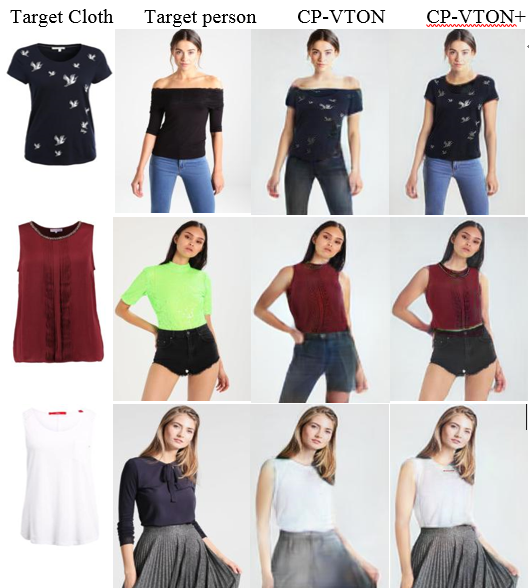
\includegraphics[height=6.5cm, scale=1]{figures/cpvton_cpvton+keyresult.png}   % TODO
%\caption{The proposed VTON results}
%\label{fig:cpvton_cpvton+keyresult}
%\end{figure}

